\documentclass{classrep}
\usepackage[utf8]{inputenc}
\usepackage{color}
\usepackage{graphicx}
\usepackage{url}
\usepackage{hyperref}

\studycycle{Informatyka, studia STACJONARNE, I st.}
\coursesemester{VI}

\coursename{Komputerowe systemy rozpoznawania}
\courseyear{2020/2021}

\courseteacher{prof. dr hab. inż. Adam Niewiadomski}
\coursegroup{poniedziałek, 12:00}

\author{
  \studentinfo{Julia Szymańska}{224441} \and
  \studentinfo{Przemysław Zdrzalik}{224466} }

\title{Projekt 2.  Podsumowania lingwistyczne relacyjnych baz danych}

\begin{document}
\maketitle

\section{Cel}
Celem projektu jest stworzenie aplikacji lingwistycznie agregującej zawartości zbioru danych wypadków samochodowych w Zjednoczonych Stanach Ameryki\cite{dane}. Jako wynik działania aplikacji zostanie wygenerowany opis zawartości danych liczbowych w zbiorze w języku quasi-naturalnym.


\section{Charakterystyka podsumowywanej bazy danych}
W programie został użyty zbiór danych\cite{dane} znajdujący się w pliku CSV, który został przekształcony w bazę danych. 

Zbiór danych zawiera informacje o ponad 3 milionach wypadków samochodowych w 49 stanach Zjednoczonych Stanów Ameryki, mających miejsce od lutego 2016 do grudnia 2020. Spośród 47 kolumn znajdujących się w zbiorze danych, wybraliśmy następujące 11 kolumn:
\begin{itemize}
\item Dotkliwość - Severity - wpływ wypadku na ruch na drodze, przyjmuje wartości całkowite od 1 do 4 włącznie, gdzie 1 oznacza najmniejszy wpływ na ruch drogowy, natomaist 4 oznacza największy wpływ. Dotkliwość można lingistycznie opisać jako mały lub duży wpływ na ruch drogowy.
\item Czas rozpoczęcia - Start\_Time - czas rozpoczęcia się wypadku w lokalnej strefie czasowej, przyjmuje wartości od 8 lutego 2016, do 31 grudnia 2020. Wartość kolumny zostanie zamieniona na wartość całkowitą oznaczającą liczbę sekund od początku 1970 roku.
\item Czas zakończenia - End\_Time - czas zakończenia się wypadku w lokalnej strefie czasowej, przyjmuje wartości od 8 lutego 2016, do 1 stycznia 2021. Wartość kolumny zostanie zamieniona na wartość całkowitą oznaczającą liczbę sekund od początku 1970 roku. 
\item Odległość - Distance - długość odcinka ulicy wyrażony w milach, na którego miał wpływ wypadek. Przyjmuje wartości zmiennoprzecinkowe od 0 do 334, gdzie zdecydowana większość danych mieści się w przedziale od 0.00 do 7.00. 
\item Temperatura - Temperature - temperatura powietrza wyrażona w Fahrenheit'ach, w momencie, gdy zdarzył się wypadek.  Przyjmuje wartości zmiennoprzecinkowe od -16.00 do 104.00.  Temperature można opisac jako bardzo zimną, zimną, umiarkowaną, ciepłą, bardzo ciepłą. Oczywiście jest to opis subiektywny.
\item Temperatura odczuwalna - Wind\_Chill - temperatura odczuwalna wyrażona w Fahrenheit'ach, w momencie, gdy zdarzył się wypadek.  Przyjmuje wartości zmiennoprzecinkowe od -16.00 do 101.00. Temperaturę odczuwalną mozna opisać tak samo jak temperaturę.
\item Wilgotność - Humidity - wilgotność powietrza wyrażona w procentach w momencie, gdy zdarzył się wypadek. Przyjmuje wartości zmiennoprzecinkowe od 4.00 do 100.00. 
\item Ciśnienie - Pressure - ciśnienie powietrza wyrażone w inches, w momencie, gdy zdarzył się wypadek. Przyjmuje wartości zmiennoprzecinkowe od 27.00 do 32.00. Ciśnieje można opisac jako wysokie, umiarkowane lub niskie. 
\item Widoczność - Visibiity - widoczność wyrażona w milach, w momencie, gdy zdarzył się wypadek. Przyjmuje wartości zmiennoprzecinkowe od 0.00 do 12.00. 
Widoczność mozna opisać jako dobrą, ograniczoną, słabą.
\item Prędkość wiatru - Wind\_Speed - prędkość wiatru wyrażona w milach na godzinę,  w momencie, gdy zdarzył się wypadek. Przyjmuje wartości zmiennoprzecinkowe od 0.00 do 40.00. Wiatr mozna opisać jako słaby, umiarkowany, silny.
\item Ilość opadów - Principation - ilość opadów wyrażona w inches, w momencie, gdy zdarzył się wypadek. Jeśli opady nie występowały to kolumna przyjmuje wartość nan.  Przyjmuje wartości zmiennoprzecinkowe od 0.00 do 0.50.
\end{itemize}
\ \\
Atrybutom nadawane są opisane zwyczajowe wartości lingwistyczne ze względu na zwiększenie przystępności i ułatwienie szybkiego zrozumienia atrybutu przez człowieka, kiedy ten atrybut nie musi być dokładnie opisany.
Przykładowo temperatura, mimo że zrozumiała dla człowieka w postaci liczbowej, jest łatwiejsza do szybszego zrozumienia w postaci tekstowej, a dla ludzi nie ma dużego znaczenia czy temperatura rózni się o 1 czy 2 stopnie, wystarczy opisać ją słownie tak jak wcześniej podaliśmy jako  bardzo zimną, zimną, umiarkowaną, ciepłą, bardzo ciepłą.


\begin{figure}[h!]
 \centering
 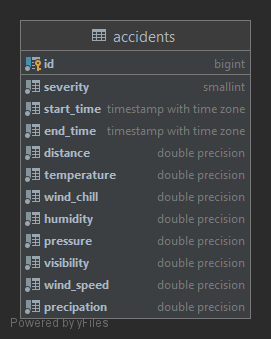
\includegraphics[width=14cm]{accidents.png}
 \vspace{-0.3cm}
 \caption{Tabela reprezentująca omawiane dane wykonana w DBMS Postgresql}
 \label{Wynik klasyfikacji.}
\end{figure}
\newpage


\section{Atrybuty i liczności obiektów wyrażone zmiennymi lingwistycznymi}
Zmienne lingwistyczne dla wybranych 10 atrybutów z bazy danych, przedstawione w
formie wykresów funkcji przynależności i wzorów analitycznych, wymienione etykiety oraz objaśnione wszystkie
symbole ułatwiające czytelnikowi ich zrozumienie \cite{zadrozny06}. Zbędne jest
cytowanie definicji. Konieczne precyzyjnie podane przestrzenie rozważań każdej
zmiennej lingwistycznej, wzory i wykresy dla każdej wartości/etykiety.\\
Jw. kwantyfikatory lingwistyczne -- opisane etykietami, wykresami funkcji
przynależności i wzorami analitycznymi. Uzasadnione wiedzą dziedzinową wybrane
zakresy i etykiety. Precyzyjnie podane przestrzenie rozważań każdego kwantyfikatora 
lingwistycznego/rozmytego, wzory i wykresy dla każdej wartości/etykiety. Opisy własne z~przypisami do literatury, tak by inżynier innej specjalności zrozumiał dalszy
opis tego konkretnego ćwiczenia/eksperymentu. \\ 
\noindent {\bf Sekcja uzupełniona jako efekt zadania Tydzień 09 wg Harmonogramu Zajęć
na WIKAMP KSR.}

\section{Narzędzia obliczeniowe: projekt (wybór, implementacja) i diagram UML pakietu obliczeń rozmytych. Diagram UML generatora podsumowań}
\subsection{Diagram pakietu obliczeń rozmytych}
Diagram UML i zwięzły opis pakietu obliczeń rozmytych: źródło pakietu
(zewnętrzny/własny/hybrydowy), przypis do literatury. Krótka charakterystyka
najważniejszych klas i podstawowych dla zadania ich metod. \\
\noindent {\bf Sekcja uzupełniona jako efekt zadania Tydzień 10 wg Harmonogramu Zajęć
na WIKAMP KSR.}

\subsection{Diagram UML generatora podsumowań. Krótka instrukcja użytkownika} 
Diagram UML generatora podsumowań (warstwy obliczeniowej oraz interfejsu
użytkownika). Krótki ilustrowany opis jak użytkownik może korzystać z aplikacji, w~szczególności
wprowadzać parametry  podsumowań, odczytywać wyniki oraz definiować własne etykiety i
kwantyfikatory. Wersja JRE i inne wymogi niezbędne do uruchomienia aplikacji przez użytkownika na własnym komputerze. \\
\noindent {\bf Sekcja uzupełniona jako efekt zadania Tydzień 11 wg Harmonogramu Zajęć
na WIKAMP KSR.}

\section{ Jednopodmiotowe podsumowania lingwistyczne. Miary jakości, podsumowanie optymalne}
Wyniki kolejnych eksperymentów wg punktów 2.-4. opisu projektu 2.  Listy podsumowań
jednopodmiotowych i tabele/rankingi podsumowań dla danych atrybutów obowiązkowe i dokładnie opisane w ,,captions'' (tytułach), konieczny opis kolumn i wierszy tabel. Dla każdego podsumowania podane miary jakości oraz miara jakości podsumowania
optymalnego.\\
\noindent {\bf Sekcja uzupełniona jako efekt zadania Tydzień 11 wg Harmonogramu Zajęć
na WIKAMP KSR.}



\section{Wielopodmiotowe podsumowania lingwistyczne i~ich miary jakości} 
Wyniki kolejnych eksperymentów wg punktów 2.-4. opisu projektu 2. Uzasadnienie i
metoda podziału zbioru danych na rozłączne podmioty. Listy podsumowań
wielopodmiotowych i tabele/rankingi podsumowań dla danych atrybutów obowiązkowe i
dokładnie opisane w ,,captions'' (tytułach), konieczny opis kolumn i wierszy tabel.
Konieczne uwzględnienie wszystkich 4-ch form podsumowań wielopodmiotowych. 
\\ 

** Możliwe sformułowanie zagadnienia wielopodmiotowego podsumowania optymalnego **.\\

{**Ewentualne wyniki realizacji punktu ,,na ocenę 5.0'' wg opisu Projektu 2. i ich porównanie do wyników z
części obowiązkowej**.}\\

\noindent {\bf Sekcja uzupełniona jako efekt zadania Tydzień 12 wg Harmonogramu Zajęć
na WIKAMP KSR.}


\section{Dyskusja, wnioski}
Dokładne interpretacje uzyskanych wyników w zależności od parametrów klasyfikacji
opisanych w punktach 3.-4 opisu Projektu 2. 
Szczególnie istotne są wnioski o charakterze uniwersalnym, istotne dla podobnych zadań. 
Omówić i wyjaśnić napotkane problemy (jeśli były). Każdy wniosek/problem powinien mieć poparcie
w przeprowadzonych eksperymentach (odwołania do konkretnych wyników: tabel i miar
jakości). Ocena które wybrane kwantyfikatory, sumaryzatory, kwalifikatory i/lub ich
miary jakości mają małe albo duże znaczenie dla wiarygodności i jakości otrzymanych
agregacji/podsumowań.  \\
\underline{Dla końcowej oceny jest to najważniejsza sekcja} sprawozdania, gdyż prezentuje poziom
zrozumienia rozwiązywanego problemu.\\

** Możliwości kontynuacji prac w obszarze logiki rozmytej i wnioskowania rozmytego, zwłaszcza w kontekście pracy inżynierskiej,
magisterskiej, naukowej, itp. **\\

\noindent {\bf Sekcja uzupełniona jako efekt zadań Tydzień 11 i Tydzień 12 wg
Harmonogramu Zajęć na WIKAMP KSR.}


\section{Braki w realizacji projektu 2.}
Wymienić wg opisu Projektu 2. wszystkie niezrealizowane obowiązkowe elementy projektu, ewentualnie
podać merytoryczne (ale nie czasowe) przyczyny tych braków. 


\begin{thebibliography}{99}
 \bibitem{niewiadomski19} A. Niewiadomski, Zbiory rozmyte typu 2. Zastosowania w reprezentowaniu informacji.  Seria „Problemy współczesnej informatyki” pod redakcją L. Rutkowskiego. Akademicka Oficyna Wydawnicza EXIT, Warszawa, 2019.
\bibitem{zadrozny06} S. Zadrożny, Zapytania nieprecyzyjne i lingwistyczne podsumowania baz danych, EXIT, 2006, Warszawa
\bibitem{niewiadomski08} A. Niewiadomski, Methods for the Linguistic Summarization of Data: Applications of Fuzzy Sets and Their Extensions, Akademicka Oficyna Wydawnicza EXIT, Warszawa, 2008.
\bibitem{dane} 2021 Kaggle Inc [internetowa społeczność związana z analizą danych], US Accidents (3 million records -- updated)
A Countrywide Traffic Accident Dataset (2016 - 2020) [przeglądany 24 kwietnia 2021], Dostępny w: \url{https://www.kaggle.com/sobhanmoosavi/us-accidents}
\end{thebibliography}

Literatura zawiera wyłącznie źródła recenzowane i/lub o potwierdzonej wiarygodności,
możliwe do weryfikacji i cytowane w sprawozdaniu. 
\end{document}
